\documentclass[14pt]{extbook}
\usepackage{multicol, enumerate, enumitem, hyperref, color, soul, setspace, parskip, fancyhdr} %General Packages
\usepackage{amssymb, amsthm, amsmath, bbm, latexsym, units, mathtools} %Math Packages
\everymath{\displaystyle} %All math in Display Style
% Packages with additional options
\usepackage[headsep=0.5cm,headheight=12pt, left=1 in,right= 1 in,top= 1 in,bottom= 1 in]{geometry}
\usepackage[usenames,dvipsnames]{xcolor}
\usepackage{dashrule}  % Package to use the command below to create lines between items
\newcommand{\litem}[1]{\item#1\hspace*{-1cm}\rule{\textwidth}{0.4pt}}
\pagestyle{fancy}
\lhead{Progress Quiz 10}
\chead{}
\rhead{Version A}
\lfoot{6232-9639}
\cfoot{}
\rfoot{Fall 2020}
\begin{document}

\begin{enumerate}
\litem{
Describe the end behavior of the polynomial below.\[ f(x) = -8(x - 4)^{4}(x + 4)^{5}(x + 9)^{3}(x - 9)^{4} \]\begin{enumerate}[label=\Alph*.]
\begin{multicols}{2}\item 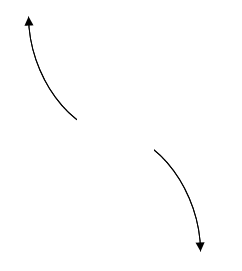
\includegraphics[width = 0.3\textwidth]{../Figures/polyEndBehaviorAA.png}\item 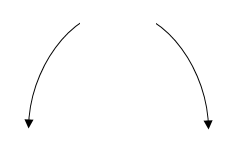
\includegraphics[width = 0.3\textwidth]{../Figures/polyEndBehaviorBA.png}\item 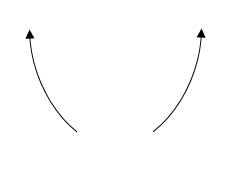
\includegraphics[width = 0.3\textwidth]{../Figures/polyEndBehaviorCA.png}\item 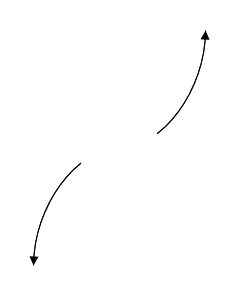
\includegraphics[width = 0.3\textwidth]{../Figures/polyEndBehaviorDA.png}\end{multicols}\item None of the above.
\end{enumerate} }
\litem{
Construct the lowest-degree polynomial given the zeros below. Then, choose the intervals that contain the coefficients of the polynomial in the form $x^3+bx^2+cx+d$.\[ -3 - 4 i \text{ and } 3 \]\begin{enumerate}[label=\Alph*.]
\item \( b \in [-1.9, 1.65], c \in [0.21, 3.58], \text{ and } d \in [-17, -10] \)
\item \( b \in [-1.9, 1.65], c \in [-0.45, 0.03], \text{ and } d \in [-10, -4] \)
\item \( b \in [-3.44, -2.63], c \in [6.39, 7.85], \text{ and } d \in [73, 79] \)
\item \( b \in [2.57, 3.6], c \in [6.39, 7.85], \text{ and } d \in [-75, -74] \)
\item \( \text{None of the above.} \)

\end{enumerate} }
\litem{
Describe the zero behavior of the zero $x = -8$ of the polynomial below.\[ f(x) = -9(x + 5)^{3}(x - 5)^{2}(x - 8)^{6}(x + 8)^{3} \]\begin{enumerate}[label=\Alph*.]
\begin{multicols}{2}\item 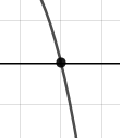
\includegraphics[width = 0.3\textwidth]{../Figures/polyZeroBehaviorCopyAA.png}\item 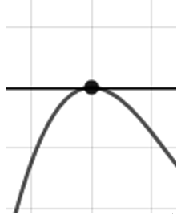
\includegraphics[width = 0.3\textwidth]{../Figures/polyZeroBehaviorCopyBA.png}\item 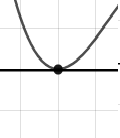
\includegraphics[width = 0.3\textwidth]{../Figures/polyZeroBehaviorCopyCA.png}\item 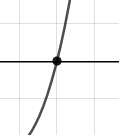
\includegraphics[width = 0.3\textwidth]{../Figures/polyZeroBehaviorCopyDA.png}\end{multicols}\item None of the above.
\end{enumerate} }
\litem{
Construct the lowest-degree polynomial given the zeros below. Then, choose the intervals that contain the coefficients of the polynomial in the form $ax^3+bx^2+cx+d$.\[ \frac{7}{5}, 5, \text{ and } \frac{3}{2} \]\begin{enumerate}[label=\Alph*.]
\item \( a \in [6, 13], b \in [-51, -48], c \in [-22, -13], \text{ and } d \in [97, 108] \)
\item \( a \in [6, 13], b \in [43, 51], c \in [-30, -22], \text{ and } d \in [-111, -103] \)
\item \( a \in [6, 13], b \in [-80, -75], c \in [161, 167], \text{ and } d \in [97, 108] \)
\item \( a \in [6, 13], b \in [-80, -75], c \in [161, 167], \text{ and } d \in [-111, -103] \)
\item \( a \in [6, 13], b \in [70, 80], c \in [161, 167], \text{ and } d \in [97, 108] \)

\end{enumerate} }
\litem{
Which of the following equations \textit{could} be of the graph presented below?
\begin{center}
    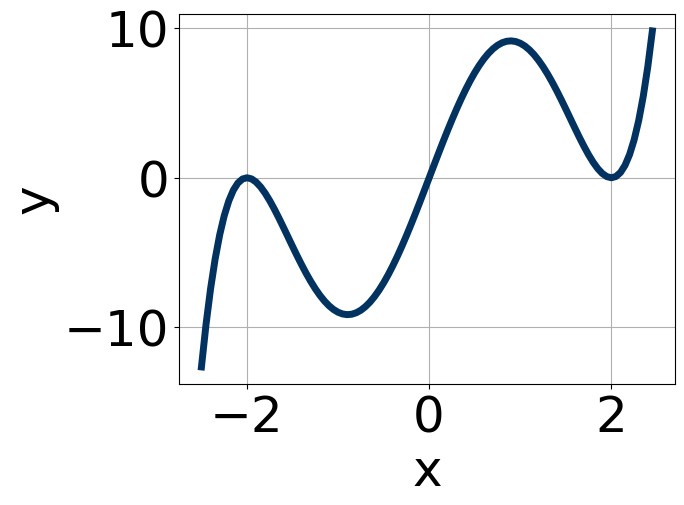
\includegraphics[width=0.5\textwidth]{../Figures/polyGraphToFunctionA.png}
\end{center}
\begin{enumerate}[label=\Alph*.]
\item \( 18x^{10} (x - 2)^{6} (x + 2)^{9} \)
\item \( 17x^{7} (x - 2)^{6} (x + 2)^{4} \)
\item \( -9x^{8} (x - 2)^{8} (x + 2)^{6} \)
\item \( 16x^{7} (x - 2)^{8} (x + 2)^{7} \)
\item \( -14x^{9} (x - 2)^{8} (x + 2)^{10} \)

\end{enumerate} }
\litem{
Describe the zero behavior of the zero $x = -3$ of the polynomial below.\[ f(x) = 7(x - 3)^{9}(x + 3)^{10}(x - 8)^{6}(x + 8)^{7} \]\begin{enumerate}[label=\Alph*.]
\begin{multicols}{2}\item 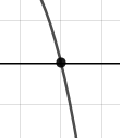
\includegraphics[width = 0.3\textwidth]{../Figures/polyZeroBehaviorAA.png}\item 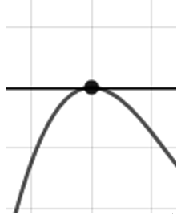
\includegraphics[width = 0.3\textwidth]{../Figures/polyZeroBehaviorBA.png}\item 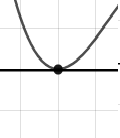
\includegraphics[width = 0.3\textwidth]{../Figures/polyZeroBehaviorCA.png}\item 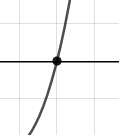
\includegraphics[width = 0.3\textwidth]{../Figures/polyZeroBehaviorDA.png}\end{multicols}\item None of the above.
\end{enumerate} }
\litem{
Describe the end behavior of the polynomial below.\[ f(x) = -9(x + 3)^{2}(x - 3)^{3}(x - 8)^{3}(x + 8)^{4} \]\begin{enumerate}[label=\Alph*.]
\begin{multicols}{2}\item 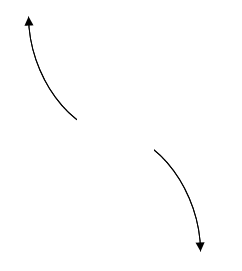
\includegraphics[width = 0.3\textwidth]{../Figures/polyEndBehaviorCopyAA.png}\item 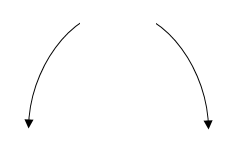
\includegraphics[width = 0.3\textwidth]{../Figures/polyEndBehaviorCopyBA.png}\item 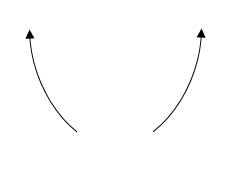
\includegraphics[width = 0.3\textwidth]{../Figures/polyEndBehaviorCopyCA.png}\item 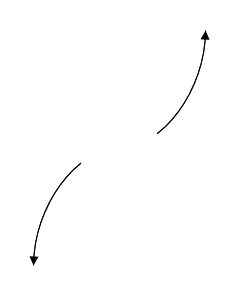
\includegraphics[width = 0.3\textwidth]{../Figures/polyEndBehaviorCopyDA.png}\end{multicols}\item None of the above.
\end{enumerate} }
\litem{
Construct the lowest-degree polynomial given the zeros below. Then, choose the intervals that contain the coefficients of the polynomial in the form $x^3+bx^2+cx+d$.\[ -2 - 5 i \text{ and } -1 \]\begin{enumerate}[label=\Alph*.]
\item \( b \in [-6.2, -3.4], c \in [31, 34.2], \text{ and } d \in [-29.2, -25] \)
\item \( b \in [-3.3, 2.4], c \in [5.7, 6.4], \text{ and } d \in [2.1, 6.8] \)
\item \( b \in [1.6, 5.7], c \in [31, 34.2], \text{ and } d \in [27.5, 30.4] \)
\item \( b \in [-3.3, 2.4], c \in [-1.2, 4.8], \text{ and } d \in [0, 3.6] \)
\item \( \text{None of the above.} \)

\end{enumerate} }
\litem{
Which of the following equations \textit{could} be of the graph presented below?
\begin{center}
    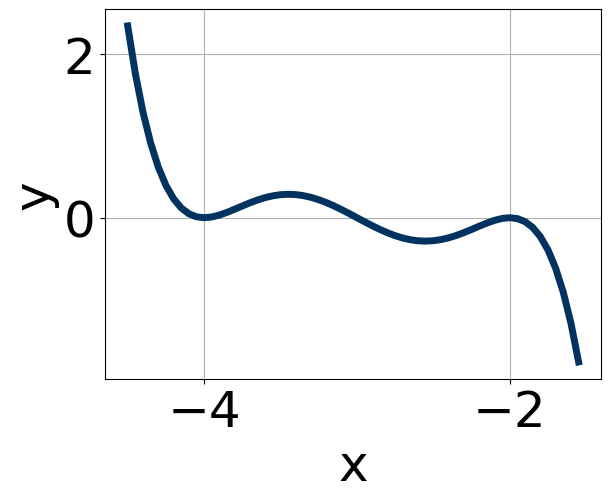
\includegraphics[width=0.5\textwidth]{../Figures/polyGraphToFunctionCopyA.png}
\end{center}
\begin{enumerate}[label=\Alph*.]
\item \( -7(x + 2)^{4} (x + 4)^{7} (x + 3)^{10} \)
\item \( 2(x + 2)^{6} (x + 4)^{6} (x + 3)^{6} \)
\item \( 20(x + 2)^{6} (x + 4)^{6} (x + 3)^{7} \)
\item \( -9(x + 2)^{6} (x + 4)^{8} (x + 3)^{11} \)
\item \( -15(x + 2)^{8} (x + 4)^{5} (x + 3)^{5} \)

\end{enumerate} }
\litem{
Construct the lowest-degree polynomial given the zeros below. Then, choose the intervals that contain the coefficients of the polynomial in the form $ax^3+bx^2+cx+d$.\[ \frac{7}{5}, \frac{-3}{4}, \text{ and } \frac{5}{3} \]\begin{enumerate}[label=\Alph*.]
\item \( a \in [60, 69], b \in [-143, -136], c \in [2, 9], \text{ and } d \in [100, 106] \)
\item \( a \in [60, 69], b \in [-69, -57], c \in [-129, -122], \text{ and } d \in [100, 106] \)
\item \( a \in [60, 69], b \in [-143, -136], c \in [2, 9], \text{ and } d \in [-109, -102] \)
\item \( a \in [60, 69], b \in [24, 32], c \in [-153, -147], \text{ and } d \in [-109, -102] \)
\item \( a \in [60, 69], b \in [138, 144], c \in [2, 9], \text{ and } d \in [-109, -102] \)

\end{enumerate} }
\end{enumerate}

\end{document}